\newpage
\section{Choosing a vision in the loop solution}

In order to create our embedded system, we have to follow some specifications: 

\begin{enumerate}
 \item The system is composed by a camera mounted on two servomotors (JIWY2) and controlled by one of this setups:
 \begin{enumerate}
  \item Combination of an Altera DE0-NANO and an Overo Fire.
  \item RaMstix extension board for Overo FireStorm-P
 \end{enumerate}
 \item The system is able to process image form the camera and move the camera in function.
\end{enumerate}

In order to follow these specifications, there are several options for the demonstration design. For example, we could have created a system that goes alternatively to different colors or try to avoid capturing a specific shape, focus on a specific color among multiple ones, etc. The underlying components for any demonstration design would remain the same (quadrature position encoders, PWM motor controllers, system stability controller with feedback) for any chosen demonstration design.\\

Based on time available for development and design complexity, a system that identifies and tracks a predefined shape with predefined color, keeping it in the centre of the view field of the camera was chosen and successfully implemented. A sample snapshot from the camera view, indicating the shape identified and the relative position of the center of the view of the camera is shown in the figure below.

\begin{figure}[!ht]
\centering
 \includegraphics[width=0.5\textwidth]{visionOnTheLoop.png}
 \caption{Our vision-on-the-loop solution}
 \label{votl}
\end{figure}


\section{System Overview}
In order for the reader to have an easier understanding of the components described further, reasoning of the choices made, and any other information included, an overview of the system implemented will be given now, with explanations followed shortly.

The base hardware platform was chosen to be RaMstix. This board has well-defined pinouts that can be quickly connected to the encoders and PWM controllers of the motors. Camera unit is fixed to communicate with the Overo Fire platform and since there is an already integrated Overo on the RaMstix board, Altera DE0-Nano was left out of the final system design. This choice is followed by using GPMC communication protocol, which has dedicated pins and routing available on the RaMstix board. GPMC protocol has pre-built implementation for both software and hardware sides, therefore its integration was rather simple and straightforward. Platform for image processing remained flexible and could be done on either side, however since frame data is first received on the Overo, this part of the system was implemented in software. The output of image processing is the position at which the center of the camera is at the moment and where it should be, based on the center of the detected object. This allows us to determine how and where camera should point, meaning that direction and speed of the motors can be calculated easily in software as well. The remaining part is sending these values to the FPGA on RaMstix, where each encoder and PWM block will receive signals corresponding to them and our camera will move as we intended.

In the table below, we present a trade-off comparison of possible solutions. This comparison assumes GPMC as the choice for the communication protocol, therefore functions in our solution space are:
\begin{itemize}
 \item Overo Fire for image capture
 \item FPGA for sending and receiving signals from JIWY2
 \item Image processing - choice between software running on NIOS II or Overo Fire
 \item Control loop - choice between software running on NIOS II or Overo Fire
\end{itemize}

Possible and feasible solutions in this case are:
\begin{itemize}
 \item NIOS+FPGA solution assumes that control loop and image processing are done on NIOS, with image capture on Overo.
 \item NIOS+Overo assumes that control loop, encoder&PWM control are done on NIOS, while Overo does image capture and image processing.
 \item Overo+NIOS assumes that control loop and image processing are done on Overo and the rest on NIOS.
 \item FPGA+Overo assumes that control loop and image processing are done on Overo without NIOS II present.
\end{itemize}

Points are given for:
\begin{itemize}
 \item Development time - how much time it takes to implement, test, and verify the design
 \item Flexibility - how configurable is the implementation
 \item Load on the platform - does this function limit or deter other functions implemented on the platform
\end{itemize}

\begin{figure}[!ht]
\hspace{-1cm}
   \centering
\begin{tabular}{|c|c|c|c|c|c|c|}\hline
            & NIOS+FPGA & NIOS+Overo &      Overo+NIOS & FPGA+Overo \\\hline
dev. time   & -++ = 2       & -++ = 2       & ++- = 2        & ++++ = 4\\\hline
flex.       & +++ = 3       & ++++ = 4      & ++++ = 4      & +++ = 3\\\hline
load        & --+ = -1      & = 0           & = 0          & +- = 0\\\hline
total       & 4         & 6          & 6          & 7\\\hline
\end{tabular}
\caption{Solutions Space evaluation}
\end{figure}

From this table, which is based on our test implementations, expectations of performance, and our skills of working with the given platform, we have decided that FPGA+Overo solution will work the best for our demonstration. 


\section{Units definition}

The first step to design such a system is  to define all the functional units we need. Each functional unit will also be divided in subsystems until we get an easy enough unit to implement it. In our case, we can define 4 units of first level: 

\begin{itemize}
 \item An encoder block that gives a feedback about the position of the camera
 \item A PWM block that control the camera movement via the servomotors
 \item An image processing block which takes picture from the camera and gets the position of the object we want to detect
 \item A control loop that translates feedback in order to make movements smoother and more stable
\end{itemize}

\begin{figure}[!ht]
\centering
 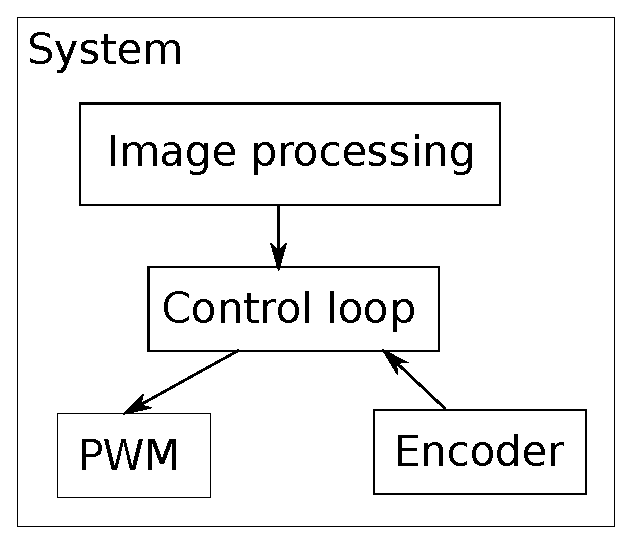
\includegraphics[width=0.5\textwidth]{dessin-1.eps}
 \caption{System schematic: High level overview}
 \label{sys_sc}
\end{figure}

To be able to design further, we know have to choose a setup and where each unit will be implemented. To help our choice, we will use some criteria and apply pondering to each criterion depending on the units working. These criteria are listed below and will be based on choices with regards to technical capabilities and limitations of certain components available in the physical setup, available development time, and skills necessary: 
\begin{itemize}
 \item Accuracy: accuracy of the final solution
 \item Implementation: easiness of implementation
 \item Flexibility: easiness of modification and correction
 \item Real-time: is the units needing a real-time execution or not
 \item Resources: calculate power and/or space needed.
\end{itemize}


\subsection{Encoder unit}

We have only relative encoder available for the camera setup, which considers an initial position and we measure movement relative to this position. The reference is not an absolute one, but will change each time we reboot the system. In order to measure movement, encoder has two rotating marked disks, partially superposed, which generate electric impulses, therefore we are able to measure movement by counting these impulses. However, if we miss even only one impulse, due to failure in the encoder or a mistake in counting, we will lose information and then get an error that will be accumulated, as we see in figure \ref{err_enc}.  

\begin{figure}[!ht]
\centering
 \includegraphics[width=0.7\textwidth]{error_encoder.png}
 \caption{Error accumulation for relative encoder}
 \label{err_enc}
\end{figure}

For this type of encoder, the main criterion is real-time, followed by accuracy, implementation, and flexibility.

\begin{figure}[!ht]
\hspace{-1cm}
\begin{tabular}{|c|c|c|c|c|c|c|}\hline
                         & Accuracy  & Implementation & Flexibility & Real-time & Resources & result \\\hline
coefficient   &         2          &           1                      &         1           &           3         &           1            &              \\\hline
FPGA            &      ++          &            +                    &         -           &        ++         &           +           &    11        \\\hline
Proc               &      ++         &              ++                &         ++       &         --          &           ++        &   4 \\\hline
\end{tabular}
\caption{trade-off table of encoder unit}
\end{figure}

\subsection{PWM unit}

PWM is used for controlling motors. The principle is to send in the direction of the motor and the speed of rotation. The direction is send by to logical wire that can respectively be set to high or low. The speed is controlled by a square periodic signal with fixed period and variable duty cycle. The speed is proportional to the average voltage and so to the duty cycle. Because we don't have any time specification for our system, hard real-time is not necessary but useful in order to avoid delay. Similarly, this unit is quite easy and shouldn't need many corrections. 

\begin{figure}[!ht]
\hspace{-1cm}
\begin{tabular}{|c|c|c|c|c|c|c|}\hline
                         & Accuracy  & Implementation & Flexibility & Real-time & Resources & result \\\hline
coefficient   &         2          &           1                      &         1           &           2         &         1               &             \\\hline
FPGA            &      ++          &            ++                 &         -           &        ++         &         +              &   10     \\\hline
Proc               &      -             &              ++               &         ++       &         --          &          ++          &       0    \\\hline
\end{tabular}
\caption{trade-off table of PWM unit}
\end{figure}

\subsection{Image processing unit}

This module is in charge to capture pictures from the camera and analyze each of them in order to detect a shape and return his position in the picture. This unit has a lot to process and have to use a driver to get data from the camera. As for PWM, because our system is not hard real-time, we still not have to much constraint about the time of the process. Furthermore, it's almost a proof of concept so that we don't need  such a good precision for our detection and we cannot really guess the final precision before implementing it. Nevertheless, we should have to configure a lot this units.

\begin{figure}[!ht]
\hspace{-1cm}
\begin{tabular}{|c|c|c|c|c|c|c|}\hline
                         & Accuracy  & Implementation & Flexibility & Real-time & Resources & result \\\hline
coefficient   &         1          &           3                      &         4           &           1         &         2               &             \\\hline
FPGA            &      n.a.        &            --                   &         --          &        n.a.       &         -              &      -16  \\\hline
Proc               &      n.a.         &            +                   &         ++        &         n.a.      &          ++          &       15    \\\hline
\end{tabular}
\caption{trade-off table of processing unit}
\end{figure}

\subsection{Control unit}

This unit is in charge to get feedback and correct send right position to the camera. This is the part that closes the loop of the system. There are a lot of controllers, more or less complex and accurate. Because of the system we want to control is quite simple, we can simply implement a proportional controller with a gain that we should be able to choose. In this case, the unit remains simple and by varying the gain, we should be able to control the system even if there is delay. An alternative is to use a sophisticated controller, based on the model representation of the physical setup in 20-sim simulation software, which then can be incorporated with the image processing unit software. Discussion on the controller is continued in its respective section \ref{controller}.

\begin{figure}[!ht]
\hspace{-1cm}
\begin{tabular}{|c|c|c|c|c|c|c|}\hline
                         & Accuracy  & Implementation & Flexibility & Real-time & Resources & result \\\hline
coefficient   &         2          &           1                      &         1           &           1         &         1               &             \\\hline
FPGA            &      +            &            +                     &         +          &          +         &         +              &   5     \\\hline
Proc               &      ++          &          ++                   &         ++       &         -           &         +              &       6    \\\hline
\end{tabular}
\caption{trade-off table of control unit}
\end{figure}

\subsection{Communication}

Another parameter to keep in mind is communication between units. Indeed, depending on which hardware we use and where we implement each unit, communication could be easier or more difficult. Communication from FPGA to FPGA is easy, as is communication from an software implemented unit to another. The difficulty is to communicate between processor and the FPGA. According to our system, the only unit that communicates with the other is the control unit. Possible choices for communication protocols are GPMC and UART. GPMC is limited to the RaMstix board, while UART can only be used between Altera DE0-Nano and Overo Fire with an external extension board. Our design was chosen to be implemented on the RaMstix board and therefore communication protocol was set as GPMC. In an overview, however, it can be seen that GPMC can be provide better flexibility over UART. Based on its structure, GPMC allows for multiple multibit registers for input and output. Main data to be transferred includes the position determined by the camera, which operates in software. Encoders will be sending live position of the camera back to controller, which is implemented in software. Position from one encoder is an 8-bit value, as well, each encoder and PWM block will require its own enable signal. On top of that, PWM blocks require duty cycle value, which is another 7 bits to be transmitted to each PWM block.\\

UART will be sending data serially, and while transmission speed, defined as baud rate, can be set very high (max of 115200 bits per second), this protocol requires setup on both sides of the transmission link. In addition to this, hardware implementation of UART on FPGA is available, but requires much more development time and can be prone to mistakes. Software implementation using NIOS II softcore IP is possible, but this method was not implemented successfully, further supporting the choice of GPMC as the main communication interface. Ability to transmit four 16-bit registers in either direction (word length can be defined to be higher, for example 32-bit to match Linux system running on Overo), allows GPMC to be a valid choice. It should also be noted that UART will be transmitting data in a specific format, which needs to repacked (unless it is done by the library, which then needs to be sourced externally, as all of the implementation of the UART). GPMC, on the other hand, allows us to put data in a specific register, addressed and accessed individually by each platform - it is clear that GPMC is the obvious choice for our design. While it wasn't measured, UART should spend about 8-9ms to transmit 1 bit (1/115200 * 1e6), but the setup requires external circuit to enable this protocol, as Altera DE0-Nano doesn't have dedicated Rx and Tx pins necesary for UART, and Over Fire requires an extender header. This external circuitry plus lengthy wires introduce the risk of faulty bits and slower data rates. GPMC is expected to be more reliable (wires routed on the PCB and are very short). In the final implementation GPMC proved to be hassle free and worked seamlessly.
